\documentclass[a4paper]{scrreprt}

%% Language and font encodings and page settings
\usepackage[english]{babel}
\usepackage[utf8x]{inputenc}
\usepackage[T1]{fontenc}
\usepackage{minted}
\usepackage[a4paper,top=2cm,bottom=2cm,left=3cm,right=3cm,marginparwidth=2cm]{geometry}
\usepackage{float}

%% Packages
\usepackage{amsmath}
\usepackage{graphicx}
\usepackage[colorinlistoftodos]{todonotes}
\usepackage[allcolors=blue]{hyperref}
\graphicspath{{./img/}}
\hypersetup{
    colorlinks=true,
    linkcolor=blue,
    filecolor=magenta,      
    urlcolor=cyan,
}

%% BibLaTeX settings
\usepackage[backend=biber]{biblatex}
\addbibresource{main.bib}

%% Header page information
\title{\href{https://github.com/cian2009/GestureBasedProject}{Project for Gesture Based UI Development}}
\subtitle{"GameFinder, a voice controlled application using the Alexa voice assistant"}

\author{
  \href{https://github.com/cian2009}{Gannon, Cian}\\
  \texttt{g00337022@gmit.ie}
  \and
  \href{https://github.com/badwulf51}{Malley O, Aron}\\
  \texttt{g00327019@gmit.ie}
}

%% Render title page
\titlehead{\centering
\includegraphics[width=10cm]{img/APP_ICON_LARGE.png}}

\begin{document}

%% Create title using header page information above
\maketitle

%% Section imports
\chapter{Purpose of the Application}
\setlength{\parskip}{1em}
The purpose of this application is to allow a user to ask for various information about games via voice commands. The user can ask many different things such as general information about the game, locations from the game as well as the different characters in the game itself. This is all done using Alexa and voice commands. For example if the user asks "what is Fallout?" Alexa will respond with information about Fallout as well as display a picture from the game. Similarly if the user asks "what is megaton?" Alexa will then respond with information about the location (Megaton) from the fallout franchise.

\begin{figure}[h!]
  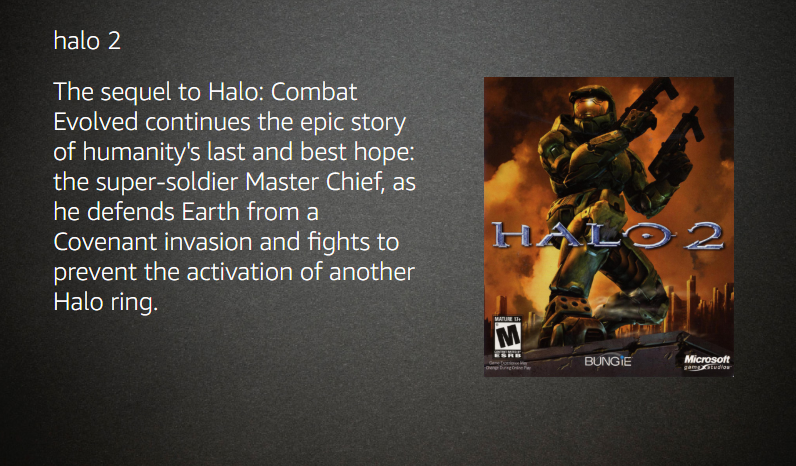
\includegraphics[width=\linewidth]{halo2.PNG}
  \caption{Game Intent}
  \label{fig:gameintent}
\end{figure}

This skill-set was made using the Giant Bomb API. Giant Bomb is a a gaming website which contains gaming related news, reviews and previews. In 2008 giant bomb created a wiki styled database to contain all the information available in the API such as characters, locations and general game knowledge. We used this API to help us create the app. 

A big part of the project was to gain better insight into how exactly gesture controls are created and what kind of gestures we should use for our given project. 

\chapter{Gestures Identified as Appropriate for this Application}
The main type of gesture used by this project is voice recognition. Listed below is the available voice commands you can use as well as what they should accomplish when said. 

\section{Gestures Used and Built Into Alexa}

\begin{enumerate}
    \item Phrase said: What is X?
    \begin{itemize}
    \item Asking "What is" followed by the name of a game will return back various basic information about the game asked. Example: What is Fallout 3?.
    \end{itemize}
    
    \item Phrase said: Who is X?
    \begin{itemize}
    \item Asking "Who is" followed by the name of a character from a game will return back various basic information about said character asked. Example: Who is Master Chief?
    \end{itemize}
    
    \item Phrase said: What is X (Location)?
    \begin{itemize}
    \item Asking "What is" followed by the name of a location from a game will return back various basic information about the location asked. Example: what is Megaton?
    \end{itemize}
\end{enumerate}

\begin{figure}[h!]
    \begin{center}
        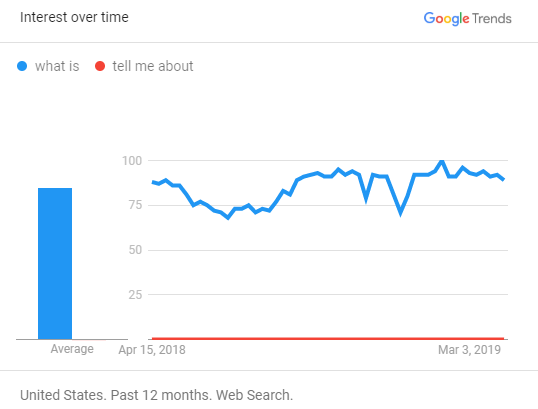
\includegraphics[width=10cm,height=10cm,keepaspectratio]{whatIsStat.png}
        \caption{Who is vs Tell me about}
        \label{fig:gameintent}
    \end{center}
\end{figure}


As you can see from the above picture during out research into what gestures we would use we looking into Google Trends to compare likely gesture that would be used by users. Using Google Trends we compared multiple gestures we thought the user might use on our Alexa skill. We compared what we thought would be the most likely option which was 'What is x?'. We then compared this gesture to others such as 'Tell me about x', in order to figure out which would be the most natural to ask our skill. Out of all the options 'What is x?' was by far the most used to ask Google a question and therefor seemed the most natural to use for our Skill.

\section{Alexa Understanding Gestures not Built-in}
Alexa works by intent, an Alexa intent works like a function would in a programming language. The intent has slots attached to it, these slots work like parameters given to the function. Intents are called by asking the skill to do a task with a given object. 'What is Fallout 3'. 'What is' is the intent and 'Fallout 3' is the object. We give the intent the 'Fallout 3' object which is laid out in the intent as a slot name. With this slot name and the given intent we can run some some of functionality.

With Alexa you program in the intents you wish Alexa to create. But Alexa works by figuring out which of the intents best match what the user is looking to use. Examples of this are 'Alexa what is Fallout 3' and 'Alexa tell me about Fallout 3'. Even though we didn't program in the intent to handle 'Tell me about' Alexa is still able to figure out which intent better matches the phrase by the user.

Tested Phrases:
\begin{enumerate}
    \item Phrase said: About X?
    \begin{itemize}
    {\item \color{green} Successful}
    \item The skill returned the information even thought the gesture wasn't built into the skill
    \end{itemize}
    
    \item Phrase said: Tell me about X?
    \begin{itemize}
    {\item \color{green} Successful}
    \item The skill returned the information even thought the gesture wasn't built into the skill
    \end{itemize}
    
    \item Phrase said: Information for x?
    \begin{itemize}
    {\item \color{green} Successful}
    \item The skill returned the information even thought the gesture wasn't built into the skill
    \end{itemize}
    
    \item Phrase said: What is x and y?
    \begin{itemize}
    {\item \color{red} Failure}
    \item This gesture was too much for the intent as it had no intent that took in two slots. This is akin to calling a function which takes in one string but instead giving it two.
    \end{itemize}
\end{enumerate}

Alexa is extremely robust in its functionality to figure out which intent best suites what the user is asking. This allowed users who had different ways of asking a question to user our skill during testing.

The gesture we built into the skill were very adjustable due to how Alexa tries to understand user intent.

\chapter{Hardware Used in Creating the Application}
During early development we looked at different hardware and software, in order to figure out what exactly we wanted to do.
We looked at the Kinect by Microsoft, Myo Armband by Elliptic Labs, Leap Motion by Leap Motion Inc and Alexa Voice Assistant by Amazon.

After looking into Myo and Kinect both had the problem were they had been discontinued. Myo has been entirely discontinued with their  website 'http://www.myo.com' is offline (Although their support site is still online for current users to download drivers). 
Kinect has been discontinued on windows and Microsoft consoles Xbox 360/One. Since the Xbox One S Microsoft have removed the port required by the Kinect and have stopped selling the adapter necessary for the Kinect to operate.

That left us with the Leap Motion and the Alexa family of devices.
We looked into what we thought would be more beneficial to learn and looked at Google trends to see which has a more Market viable skill to learn.

\begin{figure}[h!]
  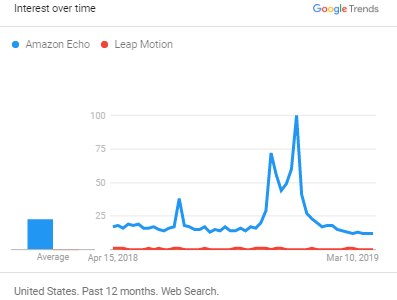
\includegraphics[width=\linewidth]{Stat.PNG}
  \caption{Google Trends}
  \label{fig:googletrends}
\end{figure}

After looking at a graph like this we can clearly see that Alexa is a more searched term over Leap Motion. With this we though that Alexa would be a better choice over Leap Motion.

\section{Echo Input - Echo Plus (Audio only)}
\begin{figure}[h!]
  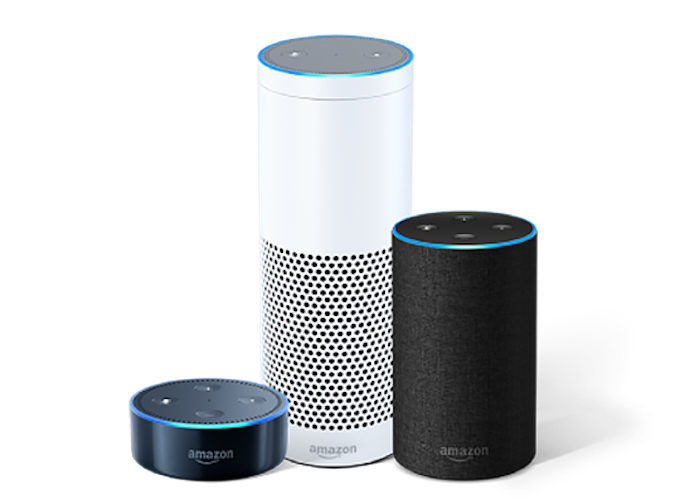
\includegraphics[width=10cm,height=10cm,keepaspectratio]{audio.png}
  \caption{Echo Audio Only}
  \label{fig:echoaudioonly}
\end{figure}

We initially started development with the intent to only develop for Echo devices with audio only, although the skill would still work on the visual models but with audio only. The entire project was built with these models in mind and only later did we add support for visual models.

\section{Echo Show \& Echo Spot (Visual)}
\begin{figure}[h!]
  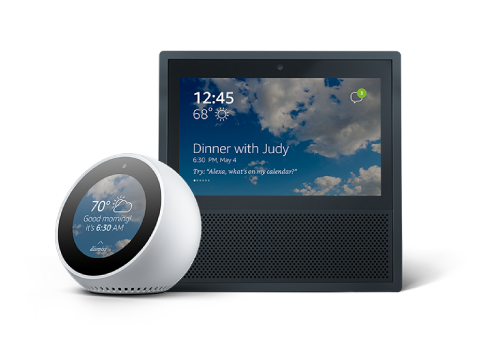
\includegraphics[width=10cm,height=10cm,keepaspectratio]{showSpot.png}
  \caption{Echo Audio Only}
  \label{fig:echoaudioonly}
\end{figure}

A the project went on an we came to terms on how exactly the Alexa voice assistant works and how it handles user interaction, we became more confident in adding more features to it. We figured out how to add a user interface by creating a basic user interface layout that we could call and add the data we needed to the user interface. This system worked very similar to how to tell Alexa to say a certain phrase, but with a few extra variables for title, text, small image and large image. Using these settings we can give more information to the user if they have an Alexa device with a screen such as the game box art.

\begin{figure}[h!]
  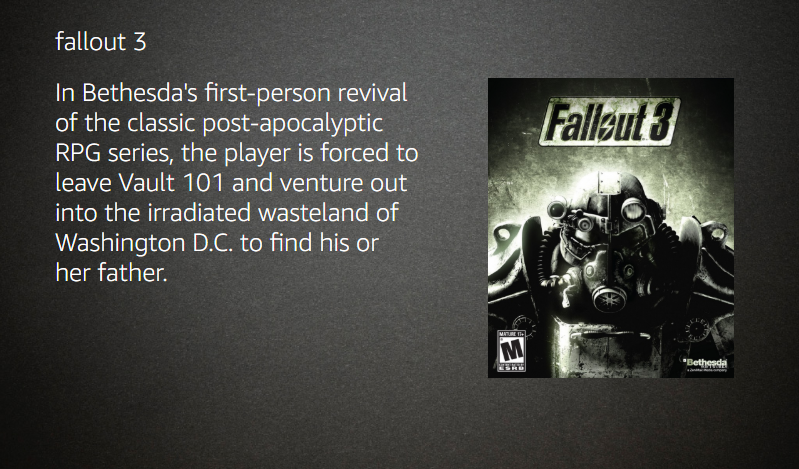
\includegraphics[width=\linewidth]{game.png}
  \caption{Game Intent}
  \label{fig:gameintent}
\end{figure}

As you see above an example of how the user interface will look when a user says 'Alexa ask game finder what is fallout 3'. The user interface will display the title of the game, a description and the game box art. We added this part to include all Alexa enabled devices on the market. Even though Alexa would still work without a user interface when we tested the skill on the Echo Show we found it didn't seem right when every other application had a user interface for these devices and ours had just audio.
\chapter{Architecture for the Solution}
\begin{figure}[h!]
  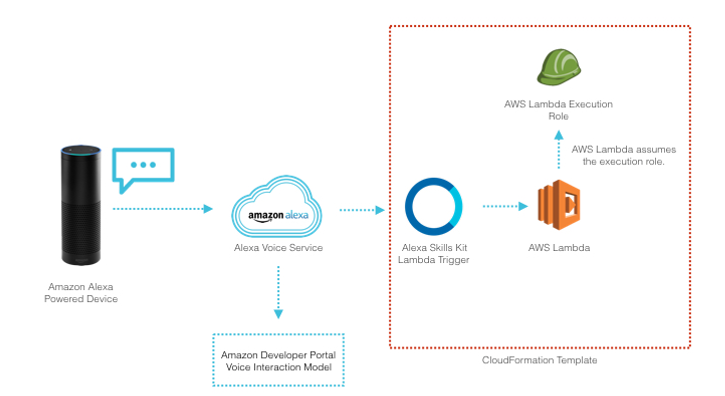
\includegraphics[width=\linewidth]{architecture.png}
  \caption{Project Architecture}
  \label{fig:projectarchitecture}
\end{figure}

Setting up the project was the hardest part of the project and much harder than we initially thought. Setting up the project involved lots of moving parts that needed to connect together and communicate from top to bottom. The project architecture involved four major parts which we will discuss in more details below. 

\section{Alexa Developer Console}
The Alexa Developer Console is where Alexa intents are stored along with the intent slots and slot types. Intents act like traditional function with slots acting as the variables part of the function. Slot types are similar to variable types where you can tell Alexa this slot (variable) is a number. This will ensure when Alexa hears 'what is one plus two' she will instead hear what is 'what is 1 plus 2', 1 and 2 being the two logs given to the function. There are many slot types for a variety of use cases such as German cities, celebrities and video games. Using these slot types Alexa will try match what the user said as best as Alexa can do a value in the given slot type.

\section{AWS Lambda}
AWS Lambda is an event-driven, server-less computing platform provided by Amazon. It saves on resources from traditional server platforms by not running at all times.
AWS Lambda will only run when the application that it is hosting is called. This saves on resources which could be very expensive for start up companies and hobby projects. AWS Lambda integrates extremely well with the Alexa Developer Console because of native support for the Lambda ARN (Amazon Resource Name) which acts as a unique link the the AWS Lambda function

\section{Project Code}
The project code is hosted on AWS Lambda which interacts with the Alexa Developer Console. The skill was programmed in Node.js.  Node.js is an open-source, cross-platform JavaScript run-time environment that executes JavaScript code outside of a browser. Node.js has great integration with AWS Lambda as it was one of the first languages supported by AWS Lambda. We picked Node.js over other languages supported by AWS Lambda because we had a bit of experience with it and we knew with the help of the NPM (Node Package Manager) we could quickly get the application to connect to the API. 

\section{GiantBomb API}
GiantBomb is an American video game website and wiki database that includes data pertaining to video games.

The GiantBomb API required a bit of setup to get working in a basic format. The API required a key which is attached to each request in order for GiantBomb to track any abuse and terminate accounts that abuse the API. We also had to add a 'device' to the HTTP request header in order for GiantBomb to track the application you are making with the API. We added the user GameFinder to the HTTP request in order to use the API by GiantBombs guidelines.










\chapter{Conclusions \& Recommendations}
Creating an Alexa for the first time was intimidating. Learning how to set up the skill was the hardest part as it was completely new to us. Learning how the Alexa skill is all wired up was a big challenge, but as time went on we figured out slowly how to get each component 'talking' with one another. Once we had each component working we rapidly were able to get the application together using Node.js. The application was hard to setup as it was out first time but easy to develop for once setup.

One of the big features of Alexa is the huge market of users it has, increasing the reach of the application. The application is hosted on \hyperlink{https://www.amazon.co.uk/Cian-GameFinder/dp/B07QH4N2GG}{Amazon UK} using the Alexa Developer Console to setup the store page. Setting up the store page worked in a very similar way to how Microsoft's Windows store works. There is a two stage verification of the application. An automatic review and a manual review. The automatic review does a basic test on the intents setup, checks if the five basic intents are setup and if the skill has the information for the store page setup. The manual review can only be done when the previous automatic review has passed. The manual review is done by an Amazon Echo employee who is given instructions by the developer on how to run the skill. The tester then tests the skill and gives feedback on how well it runs and if any changes are needed.

\begin{figure}[h!]
  
\includegraphics[width=\linewidth]{Store.PNG}
  \caption{Amazon Store}
  \label{fig:amazonstore}
\end{figure}

Once the tests were passed within a few hours the skill was live on the \hyperlink{https://www.amazon.co.uk/Cian-GameFinder/dp/B07QH4N2GG}{Amazon UK} store for free.

\begin{figure}[h!]
  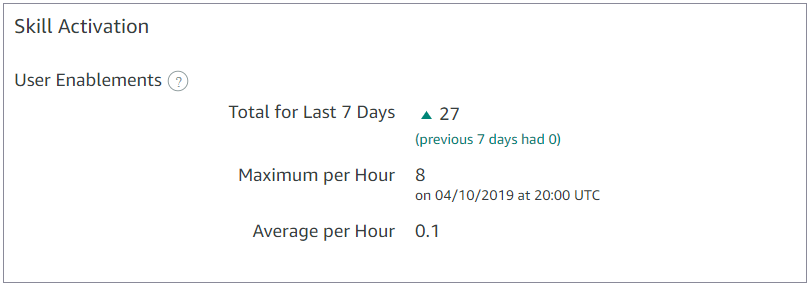
\includegraphics[width=\linewidth]{Skill.PNG}
  \caption{Amazon Store}
  \label{fig:amazonstore}
\end{figure}

Within two days we had 27 total users and 8 requests made in a single hour. We have gotten no bug reports and the AWS Lambda logs show no errors with the requests users have made.

Voice assistants have had huge growth in the last few years thank in part due to devices like the Echo and voice assistant on our phones such as Siri for IPhone and Cortana for Microsoft. Voice assistants are rapidly become a bigger part of our lives and creating an application to to get a greater understanding on how they work was very worth while.

Overall the experience in developing an Alexa skill was great. It was a completely new experience to us and we did learn a great deal more about how voice controlled assistants operate and interpret what the user say. I would recommend others to develop a gesture application using the Alexa skill framework. It's very flexible and give developers a huge market of users to get feedback from.


\end{document}